%\documentclass{article}
%\documentclass[hyperref={colorlinks=true}]{beamer}
\documentclass[handout,hyperref={colorlinks=true}]{beamer}

\usecolortheme{crane}
\usetheme{Darmstadt}
\usefonttheme{structuresmallcapsserif}
%%%%%%%%%%%%%%%%%%%%%%%%%%%%%%Paquetes%%%%%%%%%%%%%%%%%%%%%%%%%%%%%%%%%%%%%%%%%%%%%%%5
%%%%%%%%%%%%%%%%%%%%%%%%%%%%%%%%%%%%%%%%%%%%%%%%%%%%%%%%%%%%%%%%%%%%%%%%%%%%%%%%%%%%%
%\usepackage{pgfpages}
%\pgfpagesuselayout{2 on 1}[a4paper,border shrink=5mm]
\usepackage{empheq}
\usepackage[spanish]{babel}
\usepackage[utf8x]{inputenc}
\usepackage{times}
\usepackage[T1]{fontenc}
\usepackage{amssymb,amsmath}
\usepackage{enumerate}
\usepackage{verbatim}
\usepackage{ esint }
%\usepackage{pst-all}
%\usepackage{pstricks-add}
\usepackage{array}
%\usepackage[T1]{fontenc}
\usepackage{animate}
%\usepackage{media9}
\usepackage{xparse}
\usepackage{listings}
\usepackage{ wasysym }
\usepackage{sagetex}
\usepackage{yfonts,mathrsfs,eufrak}
\usepackage{hyperref}
%%%%%%%%%%%%%%%%%%%%%%%%%Configuracion listing
\lstdefinelanguage{Sage}[]{Python}
{morekeywords={False,sage,True},sensitive=true}
\lstset{
frame=none,
showtabs=False,
showspaces=False,
showstringspaces=False,
commentstyle={\ttfamily\color{dgreencolor}},
keywordstyle={\ttfamily\color{dbluecolor}\bfseries},
stringstyle={\ttfamily\color{dgraycolor}\bfseries},
language=Sage,
basicstyle={\fontsize{8pt}{8pt}\ttfamily},
aboveskip=.3em,
belowskip=0.1em,
numbers=none,
numberstyle=\footnotesize
}
%%%%%%%%%%%%%%%%%%%%%%%%Colores
\definecolor{myblue}{rgb}{.8, .8, 1}
\definecolor{dblackcolor}{rgb}{0.0,0.0,0.0}
\definecolor{dbluecolor}{rgb}{0.01,0.02,0.7}
\definecolor{dgreencolor}{rgb}{0.2,0.4,0.0}
\definecolor{dgraycolor}{rgb}{0.30,0.3,0.30}
\newcommand{\dblue}{\color{dbluecolor}\bf}
\newcommand{\dred}{\color{dredcolor}\bf}
\newcommand{\dblack}{\color{dblackcolor}\bf}
%%%%%%%%%%%%%%%%%%%%%%%%%%Nuevos comandos entornos%%%%%%%%%%%%%%%%%%%%%%%%%%%%%%%%
%%%%%%%%%%%%%%%%%%%%%%%%%%%%%%%%%%%%%%%%%%%%%%%%%%%%%%%%%%%%%%%%%%%%%%%%
\newenvironment{demo}{\noindent\emph{Dem.}}{$\square$ \newline\vspace{5pt}}
\newcommand{\com}{\mathbb{C}}
\newcommand{\dis}{\mathbb{D}}
\newcommand{\rr}{\mathbb{R}}
\newcommand{\oo}{\mathcal{O}}
\renewcommand{\emph}[1]{\textcolor[rgb]{1,0,0}{#1}}
\newcommand{\der}[2]{\frac{\partial #1}{\partial #2}}
\renewcommand{\v}[1]{\overrightarrow{#1}}
\renewcommand{\epsilon}{\varepsilon}
\newlength\mytemplen
\newsavebox\mytempbox
\makeatletter
\newcommand\mybluebox{%
\@ifnextchar[%]
{\@mybluebox}%
{\@mybluebox[0pt]}}
\def\@mybluebox[#1]{%
\@ifnextchar[%]
{\@@mybluebox[#1]}%
{\@@mybluebox[#1][0pt]}}
\def\@@mybluebox[#1][#2]#3{
\sbox\mytempbox{#3}%
\mytemplen\ht\mytempbox
\advance\mytemplen #1\relax
\ht\mytempbox\mytemplen
\mytemplen\dp\mytempbox
\advance\mytemplen #2\relax
\dp\mytempbox\mytemplen
\colorbox{myblue}{\hspace{1em}\usebox{\mytempbox}\hspace{1em}}}
\makeatother
\DeclareDocumentCommand\boxedeq{ m g }{%
{\begin{empheq}[box={\mybluebox[2pt][2pt]}]{equation}% #1%
\IfNoValueF {#2} {\label{#2}}%
#1
\end{empheq}
}%
}
\DeclareMathOperator{\atan2}{atan2}
\DeclareMathOperator{\sen}{sen}
\newtheorem{teorema}{Teorema}[section]
\newtheorem{lema}[teorema]{Lema}
\newtheorem{corolario}[teorema]{Corolario}
\newtheorem{proposicion}[teorema]{Proposici\'on}
\newtheorem{definicion}[teorema]{Definici\'on}
%%%%%%%%%%%%%%%%%%%%%%%%%%%%%%%%%%%%%%%%%%%%%%%%%%%%%%%%%%%%%%%%%%%%%%%%%%%%%%%%%%%%%%%%%%%%%%%%%%%%%%%%%%%
%%%%%%%%%%Para escibir en clase articulo o similar
% \usepackage{color}
% \newcommand{\nl}{ }
% \renewenvironment{frame}[1]{}{}
% \newcommand{\qed}{$\square$}
% %\newcommand{\defverbatim}{\def{#1}}
% \newenvironment{block}[1]{\textbf{#1}}{}
% \title{Ecuaciones lineales de segundo orden}
% \author{Fernando Mazzone}
%
%%%%%%%%%%%%%%%%%%%%%%%Para clase beamer
\newcommand{\nl}{\onslide<+-> }

\title[Teoría de Lie y ODE] % (optional, nur bei langen Titeln nötig)
{%
Teoría de Lie y ODE
}



\author[] % (optional, nur bei vielen Autoren)
{Fernando Mazzone}

\institute[Depto de Matemática] % (optional, aber oft nötig)
{
 Depto de Matemática\\
Facultad de Ciencias Exactas Físico-Químicas y Naturales\\
Universidad Nacional de Río Cuarto}


\subject{Ecuaciones Diferenciales}

%%%%%%%%%%%%%%%%%%%%%%%%%%%%%%%%%%%%%%%%%%%%%%%%%%%%%%%%%%%%%%%%%%%%%%%%%%%%%%%%%%%%%%


\begin{document}
\begin{frame}
  \maketitle
  \begin{center}
   
\includegraphics[scale=0.2]{imagenes/unrc.jpg}
   \end{center}
\end{frame}


\begin{frame}{Grupos, Repaso}
\begin{block}{Grupos}
Sean $G$ un conjunto y $\alpha$ una función tal que   $\alpha:G\times G\to G$. En el contexto de grupos es más usual la notación  $\alpha(g_1,g_2)=g_1g_2$. El par $(G,\alpha)$ se llama un grupo si se satisface
\begin{enumerate}
\item $(g_1g_2)g_3=g_1(g_2g_3)$, para todos $g_1,g_2,g_3\in G$,
\item Existe $e\in G$ tal que $eg=ge=g$,  para todo $g\in G$.
\item Para todo $g\in G$ existe $h\in G$ tal que $gh=hg=e$. Se acostumbra denotar $h=g^{-1}$.
\end{enumerate}
\end{block}


\end{frame}



\begin{frame}{Ejemplos de grupos}
\nl\textbf{Ejemplo 1} Sea $\Pi$ un plano euclideano y $G$ el conjunto de todas las transformaciones rígidas de $\Pi$ en si mismo. Entonces $G$ es un grupo con la operación de composición. Se llama el \emph{grupo de transformaciones rígidas}

\nl\textbf{Ejemplo 2} Sea $X=\{x_1,\ldots,x_n\}$ un conjunto de $n$ elementos y $S_n$ definido por 
\[S_n=\{\sigma|\sigma:X\to X\hbox{ y }\sigma \hbox{ es biyectiva }\}\]
Entonces $S_n$ es un grupo  con la operación de composición. Se denomina \href{http://es.wikipedia.org/wiki/Grupo_simétrico}{\emph{grupo simétrico}} 
\end{frame}

\begin{frame}{Ejemplos de grupos}
\nl\textbf{Ejemplo 3} Sea $\Delta$ un polígono regular de $n$ lados  en un plano euclideano $\Pi$ y $D_{2n}$ el conjunto de todas las transformaciones rígidas de $\Pi$ en si mismo que llevan $\Delta$ en si mismo. $D_{2n}$ se llama el \href{http://es.wikipedia.org/wiki/Grupo_diedral}{\emph{grupo diedral}}  de orden $2n$.
Para un triángulo equilatero
\href{http://es.wikipedia.org/wiki/Grupo_diedral}{\emph{grupo diedral}}

\begin{center}
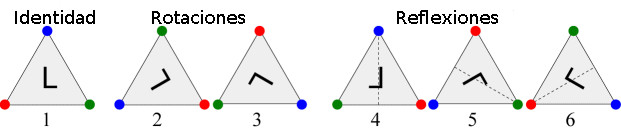
\includegraphics[scale=.4]{imagenes/SimTria.jpg}
\end{center}

\end{frame}



\begin{frame}{Teoría de grupos computacional: SAGE y GAP}

\href{http://www.gap-system.org/}{GAP - Groups, Algorithms, Programming} Lenguaje de programación para algebra discreta

\href{http://www.sagemath.org/}{SAGE:}  es un sistema de software de matemáticas libre de código abierto bajo la licencia GPL. Se basa en  muchos paquetes de código abierto existentes: NumPy, SciPy, matplotlib, SymPy, Maxima, GAP, FLINT, R y muchos más. Acceda a su poder combinado a través de un lenguaje común, basado en Python 
Misión: Creación de una alternativa libre de código abierto viable a Magma, Maple, Mathematica y Matlab.


\end{frame}

\begin{frame}[fragile]{Teoría de grupos computacional: SAGE y GAP}
\begin{sagecommandline}
sage: G=SymmetricGroup(5)
sage: sigma=G([(1,2,3),(4,5)])
sage: sigma^2
sage: sigma^3
sage: sigma^6
sage: G.order()
sage: H=G.subgroup([sigma])
sage: H.order()
\end{sagecommandline}
\end{frame}


\begin{frame}[fragile]{Teoría de grupos computacional: SAGE y GAP}
\begin{sagecommandline}
sage: H.list()
sage: H.is_normal()
sage: G1=DihedralGroup(3)
sage: G1[-2]
sage: H1=G1.subgroup(G1[-2])
sage: H1.is_normal()
sage: G1.quotient(H1)
\end{sagecommandline}
\end{frame}

\begin{frame}{Grupos de simetrías}
\nl\begin{block}{Grupos de simetrías}
Los cambios de variables de un conjunto de dos variables, digamos $x$ e $y$, son funciones $\varphi$, invertibles,  de clase $C^{\infty}$, donde $\varphi:\Omega_1\to\Omega_2$, con $\Omega_1,\Omega_2$ abiertos de $\rr^2$. Acostumbraremos escribir $(\xi,\eta)=\varphi(x,y)$ y diremos que $(\xi,\eta)$ son la variables nuevas e $(x,y)$ las viejas.

Lamaremos $\mathscr{T}$ al conjunto de todas los cambios de variables $\varphi$. 
El conjunto  $\mathscr{T}$ tiene una estructura de grupo con la operación de composición.


\end{block}


\end{frame}


\begin{frame}{Grupos de simetrías, ejemplos}
\textbf{Ejemplo, polares:} Es más facil describir la transformación que lleva coordenadas polares en cartesinas. En este caso $(x,y)=\varphi(r,\theta)$ y
\[
\begin{array}{ll}
\varphi(r,\theta)&=(r\cos(\theta),r\sen(\theta)),\\
\Omega_1&=(0,\infty)\times (-\pi,\pi),\\
\Omega_2&=\rr^2-\{(x,y)|y=0,x\leq 0\}\\
\end{array}
\]

\end{frame}

\begin{frame}{Grupos de Lie uniparamétricos}
\nl\begin{block}{Definición}
Un \href{http://es.wikipedia.org/wiki/Grupo_uniparamétrico}{\emph{grupo de Lie uniparamétrico}} es un hom,eomorfismo

\end{block}


\end{frame}

% \begin{frame}{Acción de grupos}
% \begin{block}{Acción de grupos}
% Sea $G$ un grupo   y $X$ un conjunto. Diremos que $G$ actúa a izquierda sobre $X$ si existe una función $\alpha:G\times X\to X$, denotada $\alpha(g,x)=gx$ con las propiedades
% \begin{enumerate}
% \item $ex=x$,  donde $e$ neutro de $G$ y $x\in X$.
% \item $g(hx)=(gh)x$, donde $g,h\in G$ y $x\in X$ .
% \end{enumerate}
% \end{block}

% \nl\begin{block}{Acción de grupos}
% Si $G$ actúa a izquierda sobre $X$ y $x\in X$ definimos la \emph{órbita} de $x$ como el conjunto $\{gx|g\in G\}$. Denotamos la órbita de $x$ por $Gx$.
% \end{block}
% \end{frame}




\end{document}
